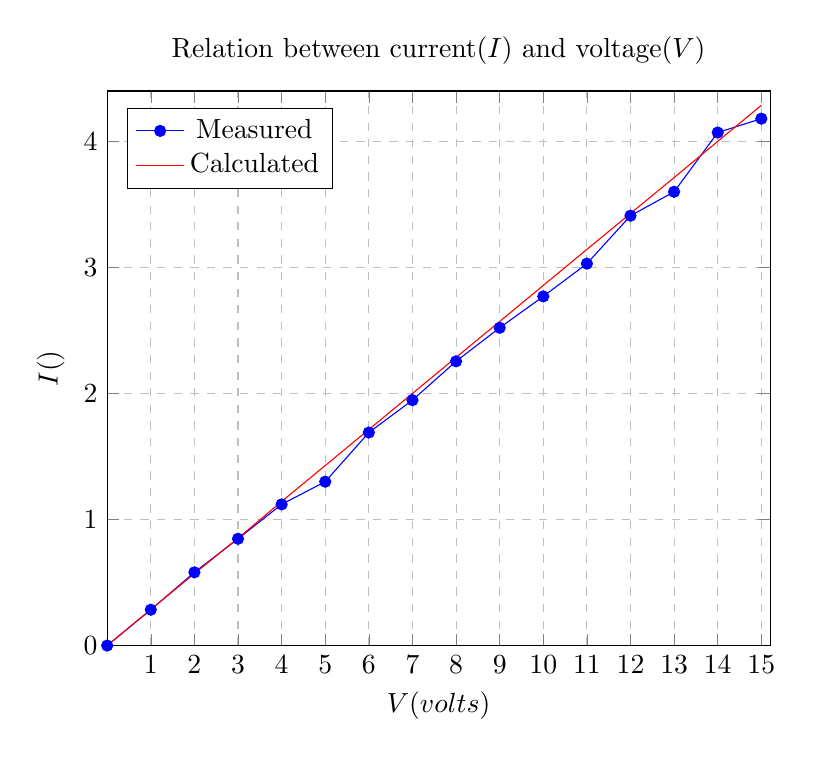
\begin{tikzpicture}
    \begin{axis}[
            title = {Relation between current($I$) and voltage($V$)},
            width=10cm,
            xlabel= {$V(volts)$},
            ylabel= {$I(\si{\milli\ampere})$},
            xmin=0,xmax=15.2,
            ymin=0,ymax=4.4,
            grid = both,
            xtick={1,2,...,15},
            grid style=dashed,
            legend pos=north west,
        ]
        \addplot[
            color=blue,
            mark=*,
        ]
            coordinates{(0,0)(1,0.284)(2,0.581)(3,0.847)
         (4,1.120)(5,1.300)(6,1.690)(7,1.947)(8,2.255)
                         (9,2.521)
                         (10,2.77)
                         (11,3.03)
                         (12,3.41)
                         (13,3.60)
                         (14,4.07)
                         (15,4.18)};
                         \addlegendentry{Measured}
        \addplot[
            mark=.,
            color=red,
        ]
            coordinates{(0,0)(1,0.287)(2,0.571)(3,0.851)
         (4,1.143)(5,1.428)(6,1.714)(7,2)(8,2.286)
                         (9,2.571)
                         (10,2.857)
                         (11,3.143)
                         (12,3.428)
                         (13,3.713)
                         (14,4)
                         (15,4.286)};
                         \addlegendentry{Calculated}
    \end{axis}         
\end{tikzpicture}      
